During the spring semester, we will work on three macro-areas: platform development, platform evaluation, and report writing.
A drilled-down list of the aforementioned macro-areas can be found in the next section of this proposal (Section~\ref{sec:work-plan-for-the-spring-semester}). \\ \\
The architecture of API Scout is defined in Figure~\ref{fig:platform-architecture}.
\begin{figure}
    \centering
    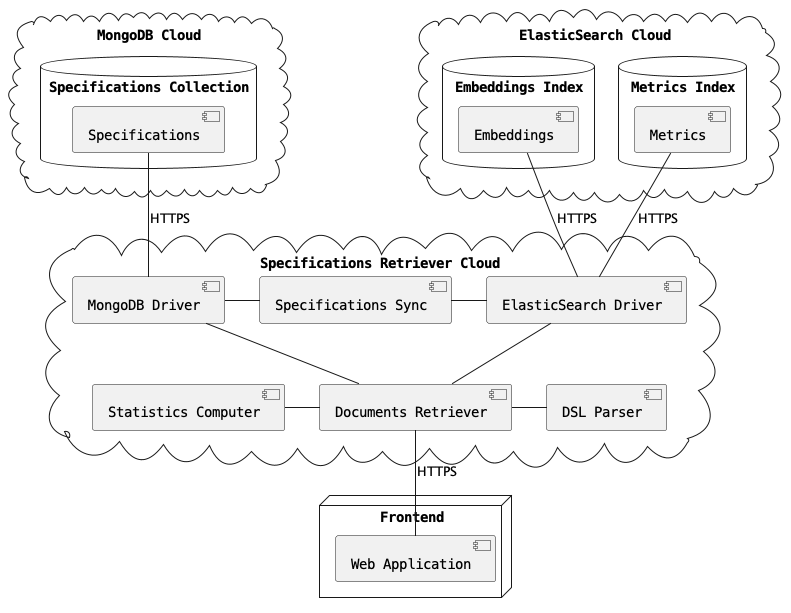
\includegraphics[width=10cm]{/Users/edoriggio/Documents/USI/github/thesis/research/out/pumls/deployment}
    \caption{API Scout Architecture}
    \label{fig:platform-architecture}
\end{figure}
The system will be divided into four main parts: the ElasticSearch cloud, the MongoDB cloud, the backend, and the frontend.
\begin{description}
    \item[ElasticSearch Cloud] This part of the system will contain two indices, one for the embeddings of the OpenAPI specifications, and one for the pre-computed metrics of the OpenAPI specifications.
    \item[MongoDB Cloud] This part will contain one collection containing all the $\sim$500k scraped OpenAPI specifications.
    \item[Backend] This part of the system performs all the necessary operations on the databases and exposes an HTTP API to the frontend.
    More specifically, it will keep the two databases in sync, parse the DSL passed from the frontend, compute on-the-fly statistics given a user-defined query, and finally it retrieves the documents that are most similar to the given query (Subsection~\ref{subsec:approach}).
    \item[Frontend] This last part will handle all the user interaction with the collection of OpenAPI specifications.
    The user will be able to search the collection, as well as visualize the structure of the specification and analyze the evolution of a given API through time.
\end{description}
